% Created 2020-04-17 Fri 00:14
% Intended LaTeX compiler: pdflatex
\documentclass{article}
\usepackage[utf8]{inputenc}
\usepackage[T1]{fontenc}
\usepackage{graphicx}
\usepackage{grffile}
\usepackage{longtable}
\usepackage{wrapfig}
\usepackage{rotating}
\usepackage[normalem]{ulem}
\usepackage{amsmath}
\usepackage{textcomp}
\usepackage{amssymb}
\usepackage{capt-of}
\usepackage{hyperref}
\date{\today}
\title{}
\hypersetup{
 pdfauthor={},
 pdftitle={},
 pdfkeywords={},
 pdfsubject={},
 pdfcreator={Emacs 26.3 (Org mode 9.3.6)}, 
 pdflang={English}}
\begin{document}

\tableofcontents

\section{Algorithm/Code}
\label{sec:org3d7fe47}
\begin{enumerate}
\item Whoel Porgram decompsiostion
\label{sec:org2e4086f}
This is an outline/code of how the whole program will be. 
\item Bit Parsing/Data Strucutre\hfill{}\textsc{BIT}
\label{sec:org30ec858}
\begin{itemize}
\item As we are writing bits, we have to format the disk to be able to read and write bits.
\item SUPERBLOCK | indoebitmap | datablock bitmap | sequence of indoes | sequence of datablcoks = 1000
\item the sequence of indoes will ahve 3 sectors, due to each indoe being able to represtn 35 inodes.
\item The rest of the space, 994 sectors, are for teh databock block.
\end{itemize}

\begin{enumerate}
\item inode
\label{sec:org4236d70}
\begin{description}
\item{writeBitStream()} Write teh type, size and allociation, by reversing the blwo opeariton

\item{readBitStream()} read the type, size and allcioation by folowing the following processess

\item There are 4 indoes within a inode sector. The makeup totals to 114 bits.
\begin{description}
\item{1 bit } for which type of inode this is.
\item{13 bits} (or 1.625 bytes) for representing the size of datablocks
\item{100 bits} 10 seqeunces of 10 bits for reprsenting the location. note that all 1s mean that this is not allociated
\end{description}

\item This results of 106 of useless data, and 3990 of useful data. Since there are 35 inodes in a sector, we split it up into an array, with each piece being a substr of 114 bits.

\item The function below is a method ofreading it. Note it doesn't return anything. Maybe i'll try to do that thing where i have an inlnie function and do it there.

\item Anotehr note: there'll be 35 inodes withn a sector, so the spliting of that by 114 is left to futrue zak.

\item Writing it to bitstream is simple. if need be write a funciton for it.
\end{description}


\item datablock
\label{sec:org91ec5ff}
\begin{itemize}
\item Datablocks are disgshiustehd by two types: file and directory
\item the type of the datablock is denoted by teh inode, not the directory.
\item For directory, tehre is a 20 bytes/160 bits, which are
\begin{description}
\item{16 bytes/128 bits} file name. 15 characters PLUS 1 for end of string, so it's mroe of 15 characters
\item{4 byte/32 bits} inode that shows which file/driectory this is.
\end{description}
\item This means that dictionaries cna have 25 files in a a sector, but 250 files/directories overall.
\item This doesn't have the case, of half a directoriy's infroamtion being in one datablcok, and the other half being in another datablock. THat isn't consdiered.
\begin{verbatim}
using namespace std;
void readDir(string TestString){
    bitset<4> inode(TestString.substr(0,4));
    cout << inode.to_ulong() << endl;
    char temp[10];
    for(int i=0; i<16; i++){
	    bitset<8> temp(TestString.substr(4+i*8,8));
	    cout << (char)temp.to_ulong() << endl;

    }

}

int main(){
/*
	string temp1="iiii11111111111111112222222222222222333333333333333344444444444444445555555555555555666666666666666677777777777777778888888888888888";
	for(int i=0; i<8; i++){
	    cout << temp1.substr(4+i*16,16) << endl;
	}
*/
	/*readDir("111110000000000000001000000000000000100000000000000010000000000000001000000000000000100000000000000010000000000000001000000000000000");*/
       readDir("111101000001010000100100001101000100010001010100011001000111010010000100000101000010010000110100010001000101010001100100011101001000");
       /*
       111101000001010000100100001101000100010001010100011001000111010010000100000101000010010000110100010001000101010001100100011101001000*/
}

\end{verbatim}
\end{itemize}

\item bitmap of indoe/datablock
\label{sec:org1f661cd}
\begin{itemize}
\item this is just a bitmap, used to keep trakc of which indoes are allociated and which datablocks are allociated.
\end{itemize}
\item Sector/Root Inode
\label{sec:orgead8b12}
\begin{itemize}
\item A sector is a collection of a superblock, bitmaps for in use indoes and datablocks, a sqeunce of indoes, and a sequence of datablocks.  However, this information HAS TO BE CONVERETD to that. Otehrwise, a sector is just an array of bitsets of 4096 bits.
\item However, the sector converts it's concats to usuable datasturcutres. After each file/directory operation, it saves the stuff to workign directory. Than, working directory saves it stuff to external disk when FS\textsubscript{SYNC}() is made.
\item The disks are just a bitset array of 4096 bits, with 1000 elements in each.
\item The root inode is the indoe that represtns nothing. This is a special variable, as to not have to find out what it is on disk tediously.
\end{itemize}

\begin{verbatim}
std::bitset<4096> ExtDisk[1000];
std::bitset<4096> WorkDisk[1000];
\end{verbatim}
\end{enumerate}

\item File System\hfill{}\textsc{FS}
\label{sec:orgeb8bde6}
\begin{description}
\item{FS\textsubscript{BOOT}()} Called when booting filesystem/after a FS\textsubscript{RESET}()
\begin{center}
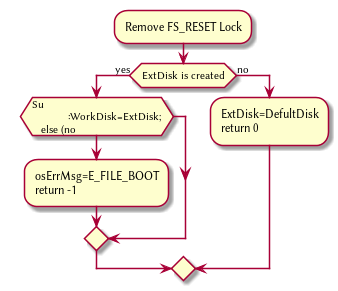
\includegraphics[width=.9\linewidth]{Plant/FS_BOOT.png}
\end{center}
]

\item{FS\textsubscript{Sync}} Copys the working disk to external disk
\begin{center}
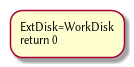
\includegraphics[width=.9\linewidth]{Plant/FS_SYNC.png}
\end{center}

\item{FS\textsubscript{RESET}()} Stops the filesystem from ebing access, by placing a lock on it. 
\begin{center}
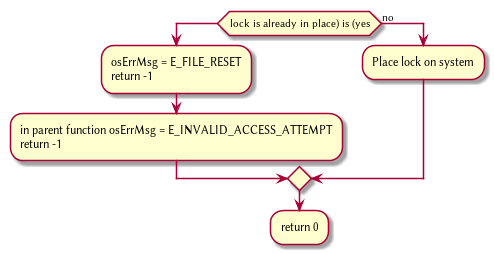
\includegraphics[width=.9\linewidth]{Plant/FS_RESET.png}
\end{center}
\end{description}

\item File Access\hfill{}\textsc{FILE}
\label{sec:org4c03370}
\begin{description}
\item{int getInode(string path)} Helper function, used to get the inode given a path.
\begin{description}
\item{Ouptut} inode number of where it is, or -1 if it's not found.
\begin{center}
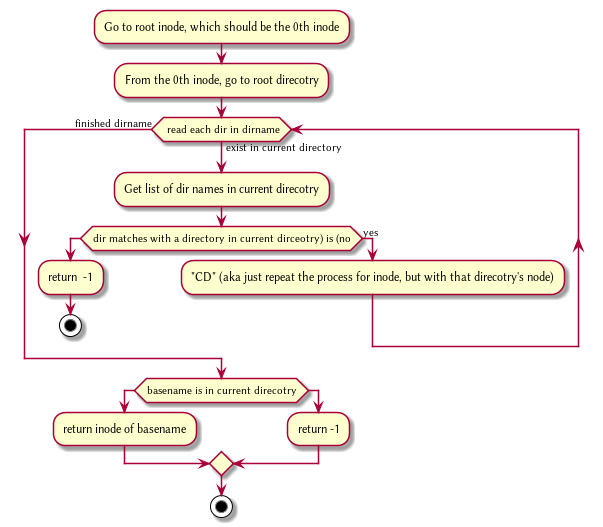
\includegraphics[width=.9\linewidth]{Plant/getInode.png}
\end{center}
\end{description}

\item{int getInode(string path)} Helper function, used to get the file given a path.
\begin{description}
\item{Ouptut} inode number of where it is, or -1 if it's not found.
\begin{center}
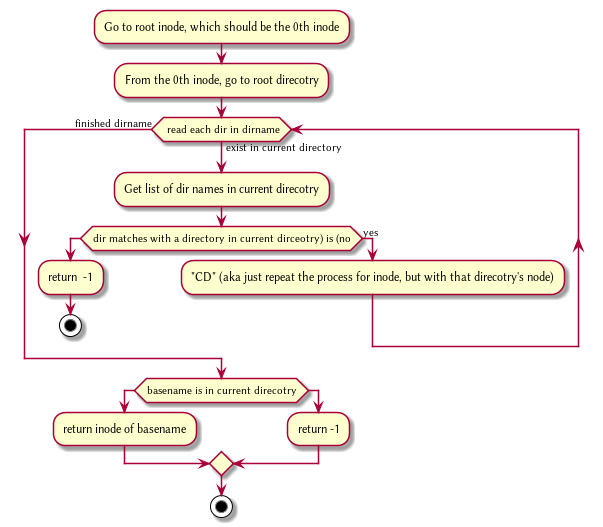
\includegraphics[width=.9\linewidth]{Plant/getInode.png}
\end{center}
\end{description}

\item{File\textsubscript{Create}(string path)} Create a new file at path. There is a check to see if that file already exist, and if there's a free datablock for it.
\begin{center}
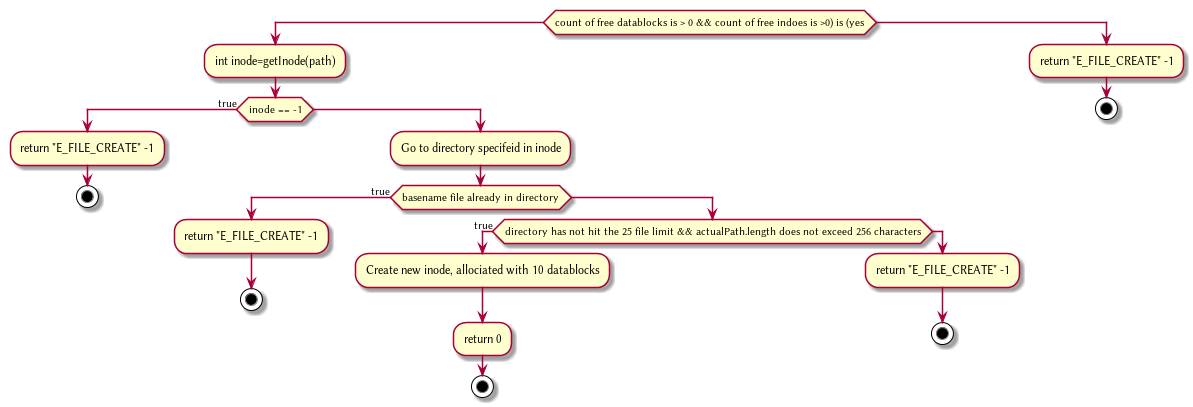
\includegraphics[width=.9\linewidth]{Plant/FileCreate.png}
\end{center}
\end{description}


\begin{description}
\item{File\textsubscript{Open}(string path)} returns the file descriptor of the file, which can be used to read and write to it.
\begin{center}
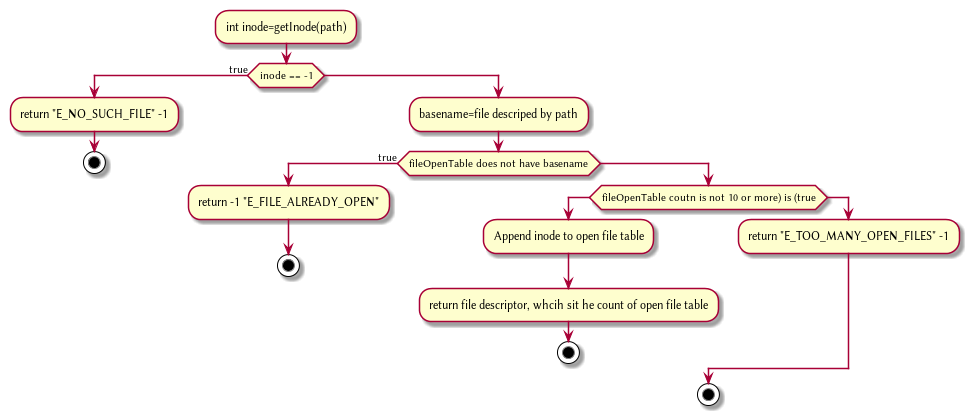
\includegraphics[width=.9\linewidth]{Plant/FileOpen.png}
\end{center}
\item{File\textsubscript{Read}(int fd, string buffer, int size IN BYTES)} Buffer reads size from the file in fd. Note the file in open file table shuold move by size
\begin{center}
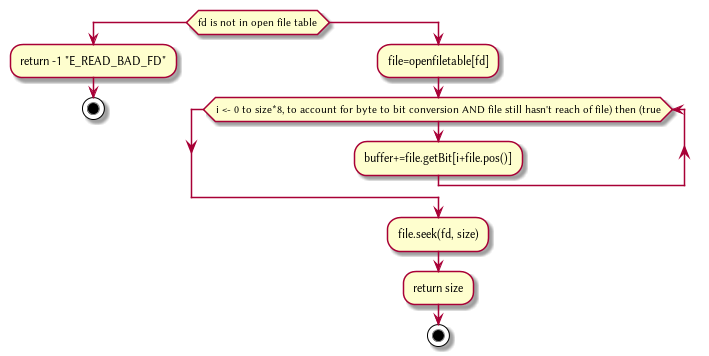
\includegraphics[width=.9\linewidth]{Plant/FileREAD.png}
\end{center}
\item{File\textsubscript{Write}(int fd, string buffer, int size IN BYTES)} Write from buffer to the file. NOTE SIZE HAS TO BE CONSISNET. If it's not, stop the program
\begin{center}
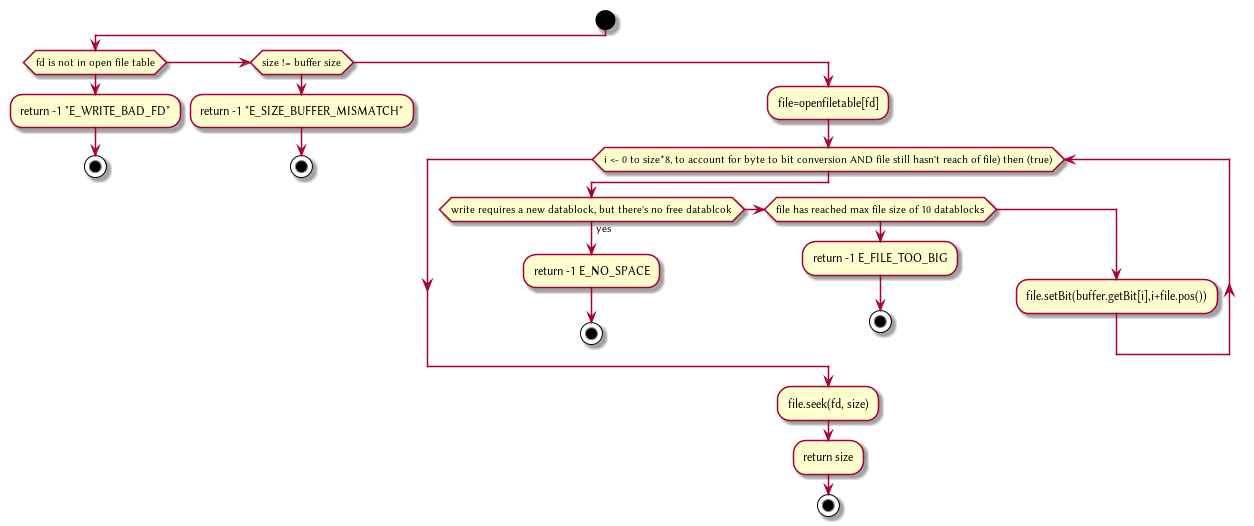
\includegraphics[width=.9\linewidth]{Plant/FileWrite.png}
\end{center}

\item{File\textsubscript{Seek}(int fd, int offset)} move the file forward  by offset.
\begin{center}
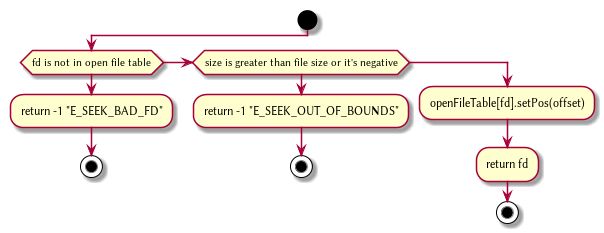
\includegraphics[width=.9\linewidth]{Plant/FileSeek.png}
\end{center}

@startuml

\begin{center}
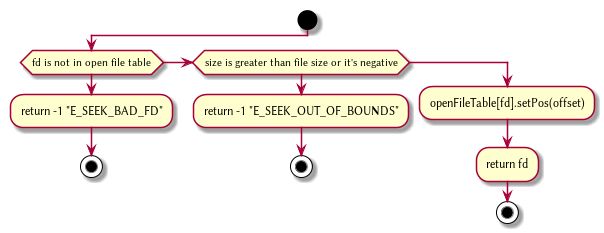
\includegraphics[width=.9\linewidth]{Plant/FileSeek.png}
\end{center}
\item{File\textsubscript{Close}(int fd)} Remove file from table
\begin{center}
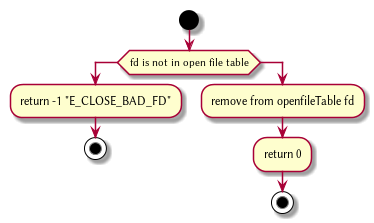
\includegraphics[width=.9\linewidth]{Plant/FileClose.png}
\end{center}

\item{File\textsubscript{UnLink}(string path)} Delete file from the filesystem.
\begin{center}
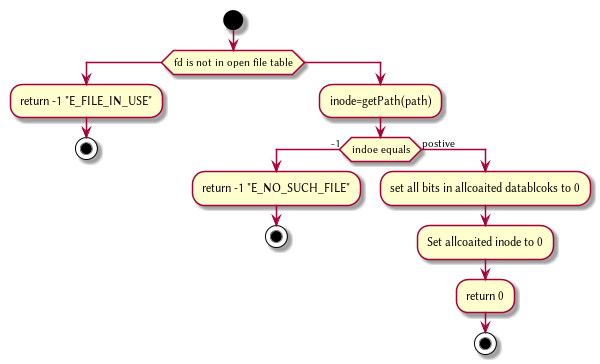
\includegraphics[width=.9\linewidth]{Plant/FileDelete.png}
\end{center}
\end{description}

\item Directory\hfill{}\textsc{DIR}
\label{sec:org57ef08b}
\begin{description}
\item{Dir\textsubscript{Create}(string path)} Create directory at path
\begin{center}
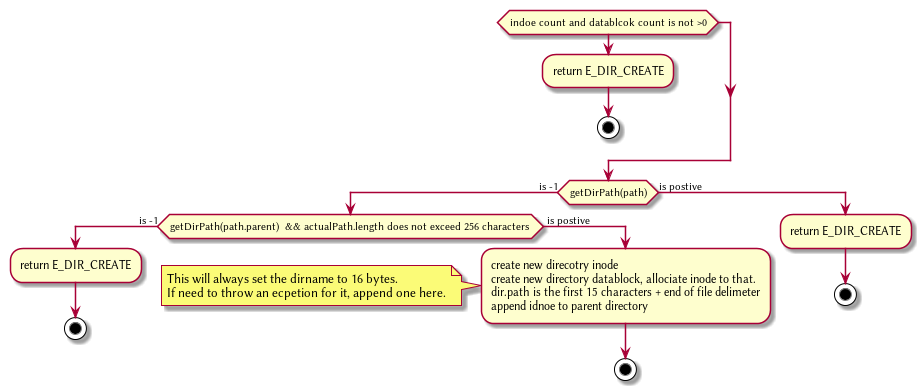
\includegraphics[width=.9\linewidth]{Plant/DirCreate.png}
\end{center}

@startuml

\item{Dir\textsubscript{Read}(string path, string buffer, itn size)} Read the contents of a directory.
\begin{center}
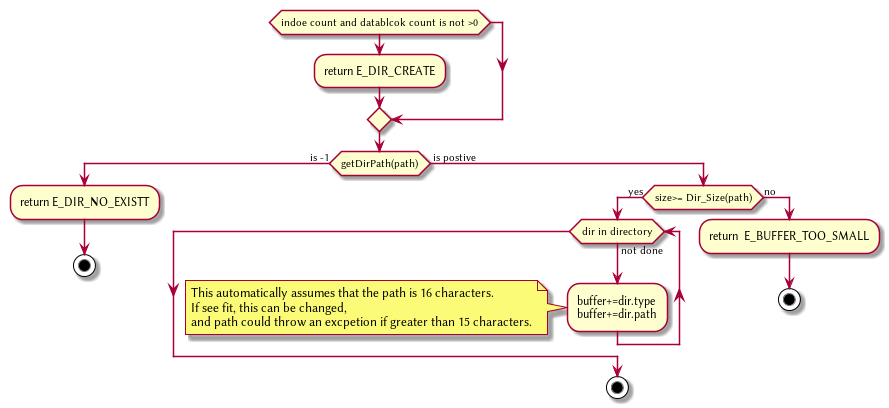
\includegraphics[width=.9\linewidth]{Plant/DirRead.png}
\end{center}
\item{Dir\textsubscript{Unlink}(string path)} Remove file from drive
\begin{center}
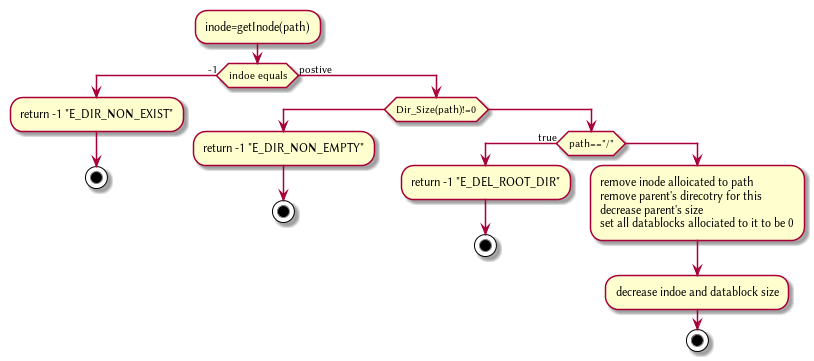
\includegraphics[width=.9\linewidth]{Plant/DirUnlink.png}
\end{center}
\end{description}

\item Disk\hfill{}\textsc{DISK}
\label{sec:org3454b42}

\begin{description}
\item{DISK\textsubscript{INIT}()} Set all the data in the disk to be 0
\begin{center}
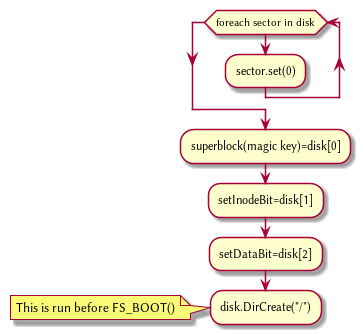
\includegraphics[width=.9\linewidth]{Plant/DIskInit.png}
\end{center}

\item{DISK\textsubscript{LOAD}()} Save external disk to workign disk. Done when booting. 

\begin{center}
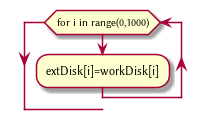
\includegraphics[width=.9\linewidth]{Plant/DIskLoad.png}
\end{center}

\item{DISK\textsubscript{SAVE}()} Save working disk to loading. Called by FS\textsubscript{SYNC}()
\end{description}
\begin{center}
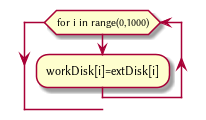
\includegraphics[width=.9\linewidth]{Plant/DIskSave.png}
\end{center}

\begin{description}
\item{DISK\textsubscript{WRITE}(int sector, string buffer)} Write from buffer to disk.

\begin{center}
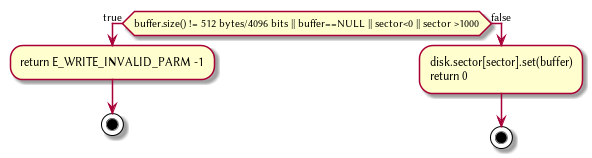
\includegraphics[width=.9\linewidth]{Plant/DiskWrite.png}
\end{center}
\end{description}



\begin{description}
\item{DISK\textsubscript{Read}(int sector, string buffer)} read from sector to buffer

\begin{center}
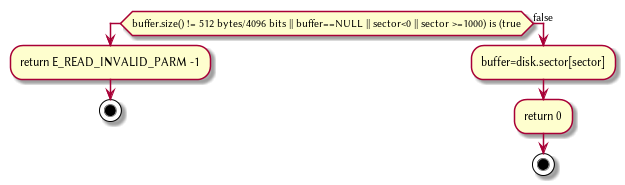
\includegraphics[width=.9\linewidth]{Plant/DiskREAD.png}
\end{center}
\end{description}
\end{enumerate}
\end{document}